% Sprawozdanie SIGK, Projekt 1. Kompilacja: latexmk -xelatex sprawozdanie.tex
% Rysunki: python docs/sprawozdanie/make_figures.py (z katalogu projektu).
\documentclass[11pt,a4paper]{article}

\newcommand{\autorPierwszy}{Kacper Preyzner}
\newcommand{\autorDrugi}{Rafał Zwierzyński}

\usepackage{fontspec}
\usepackage{polyglossia}
\setdefaultlanguage{polish}
\usepackage{unicode-math}
\setmainfont{LibertinusSerif}[Extension=.otf, UprightFont=*-Regular, BoldFont=*-Semibold,
  ItalicFont=*-Italic, BoldItalicFont=*-SemiboldItalic]
\setsansfont{LibertinusSans}[Extension=.otf, UprightFont=*-Regular, BoldFont=*-Bold,
  ItalicFont=*-Italic]
\setmonofont{LibertinusMono}[Extension=.otf, UprightFont=*-Regular, Scale=0.92]
\setmathfont{LibertinusMath-Regular.otf}

\usepackage[a4paper,margin=2.4cm,top=2.2cm,bottom=2.6cm]{geometry}
\usepackage{microtype}
\usepackage{graphicx}
\usepackage{booktabs}
\usepackage{tabularx}
\usepackage{multirow}
\usepackage{array}
\usepackage[table]{xcolor}
\usepackage{siunitx}
\usepackage{caption}
\usepackage{enumitem}
\usepackage{csquotes}
\usepackage{fancyhdr}
\usepackage{titlesec}
\usepackage{float}
\usepackage{tikz}
\usetikzlibrary{arrows.meta,positioning,fit,calc,backgrounds}
\usepackage{pgfplots}
\usepgfplotslibrary{groupplots}
\pgfplotsset{compat=1.18}
\usepackage[hidelinks]{hyperref}

\definecolor{akcent}{HTML}{1F4E79}
\definecolor{jasny}{HTML}{EAF1F8}
\definecolor{siec}{HTML}{C0504D}
\definecolor{baza}{HTML}{7F7F7F}

\sisetup{output-decimal-marker={,}, group-separator={\,}, group-minimum-digits=4, group-digits=integer,
  detect-weight=true, detect-family=true}
\captionsetup{font=small, labelfont={bf,color=akcent}, labelsep=period, skip=6pt}
\captionsetup[table]{position=top}
\setlist{itemsep=2pt, topsep=4pt}
\setlength{\parskip}{3pt}
% Bez pakietu texlive-langpolish (wzorce dzielenia) dajemy łamaniu więcej swobody.
\setlength{\emergencystretch}{3.5em}
\tolerance=1500
\renewcommand{\arraystretch}{1.15}

\titleformat{\section}{\Large\sffamily\bfseries\color{akcent}}{\thesection}{0.6em}{}
\titleformat{\subsection}{\large\sffamily\bfseries\color{akcent}}{\thesubsection}{0.6em}{}
\titlespacing*{\section}{0pt}{14pt}{6pt}
\titlespacing*{\subsection}{0pt}{10pt}{4pt}

\pagestyle{fancy}
\fancyhf{}
\fancyhead[L]{\small\sffamily\color{baza} SIGK -- Projekt 1: Modyfikacja obrazów}
\fancyhead[R]{\small\sffamily\color{baza} \autorPierwszy, \autorDrugi}
\fancyfoot[C]{\small\sffamily\thepage}
\renewcommand{\headrulewidth}{0.4pt}

\newcommand{\code}[1]{\texttt{\mdseries #1}}
\newcommand{\best}[1]{\textbf{#1}}
\newcommand{\nazwa}{ResidualNet}

\begin{document}

% ---------------------------------------------------------------- strona tytułowa
\begin{titlepage}
  \begin{tikzpicture}[remember picture, overlay]
    \fill[akcent] (current page.north west) rectangle ([yshift=-5.2cm]current page.north east);
    \node[anchor=west, text=white, font=\sffamily\large] at ([xshift=2.4cm,yshift=-2.0cm]current page.north west)
      {Sztuczna Inteligencja w Grafice Komputerowej};
    \node[anchor=west, text=white, font=\sffamily\Huge\bfseries] at ([xshift=2.4cm,yshift=-3.2cm]current page.north west)
      {Projekt 1: Modyfikacja obrazów};
  \end{tikzpicture}
  \vspace*{5.2cm}

  \noindent{\sffamily\LARGE Zwiększanie rozdzielczości i odszumianie obrazów\\[2pt]
   siecią rezydualną \nazwa\par}
  \vspace{0.8cm}
  \noindent{\large\sffamily Sprawozdanie z realizacji projektu\par}
  \vspace{1.6cm}

  \noindent\begin{tabular}{@{}ll@{}}
    \sffamily\bfseries Zespół: & \autorPierwszy \\
                               & \autorDrugi \\[6pt]
    \sffamily\bfseries Wybrane zadania: & 2.1 Zwiększanie rozdzielczości, 2.2 Odszumianie \\
  \end{tabular}

  \vfill
  \noindent\colorbox{jasny}{\parbox{\dimexpr\textwidth-2\fboxsep}{\small
    \textbf{W skrócie.} Zrobiliśmy dwa z czterech zadań: zwiększanie rozdzielczości
    ($64\times64\to256\times256$ oraz $32\times32\to256\times256$) i odszumianie
    (szum gaussowski $\sigma=0{,}01$ i $0{,}03$). Do obu zadań użyliśmy tej samej, małej sieci
    rezydualnej, która uczy się \emph{poprawki} do obrazu wejściowego. Na 100 obrazach testowych
    sieć była lepsza od metod bazowych (bicubic z OpenCV i \code{denoise\_bilateral} ze scikit-image)
    w każdym z czterech wariantów i w każdej metryce: SNE, PSNR, SSIM i LPIPS. Przy odszumianiu
    zysk PSNR wyniósł $+3{,}8$ i $+4{,}7$~dB, a przy zwiększaniu rozdzielczości $+0{,}7$ i $+0{,}5$~dB.}}
\end{titlepage}

\tableofcontents
\vspace{0.6cm}

% ---------------------------------------------------------------- 1
\section{Cel projektu i wybór zadań}

Zgodnie z instrukcją mieliśmy zaproponować architekturę sieci neuronowej, wykorzystać ją do
dwóch z czterech zadań modyfikacji obrazów i porównać wyniki z metodami bazowymi przy pomocy
metryk z wykładu. Wybraliśmy:
\begin{itemize}
  \item \textbf{zwiększanie rozdzielczości} (super-resolution, SR) z obrazów $64\times64$ (powiększenie
        $\times4$) i $32\times32$ (powiększenie $\times8$) do $256\times256$,
  \item \textbf{odszumianie} obrazów z addytywnym szumem gaussowskim o $\sigma=0{,}01$ i $\sigma=0{,}03$.
\end{itemize}

Oba zadania pasują do wspólnego modelu degradacji z wykładu W04, $y = D(x) + n$: przy SR operacja
$D$ to zmniejszenie rozdzielczości, a przy odszumianiu $D$ jest identycznością i zostaje tylko szum $n$.
Dlatego mogliśmy użyć jednej rodziny sieci, zmieniając tylko końcowy moduł powiększania.
Dla każdego z czterech wariantów (\code{sr4}, \code{sr8}, \code{dn001}, \code{dn003}) wytrenowaliśmy
osobny model.

Tabela~\ref{tab:wymagania} zestawia wymagania z instrukcji z miejscami, w których opisujemy ich realizację.

\begin{table}[H]
  \centering\small
  \caption{Wymagania z instrukcji i ich realizacja.}
  \label{tab:wymagania}
  \begin{tabularx}{\textwidth}{@{}>{\raggedright\arraybackslash}p{4.6cm}X>{\centering\arraybackslash}p{1.4cm}@{}}
    \toprule
    Wymaganie & Realizacja & Sekcja \\
    \midrule
    Python + PyTorch & cały kod w pakiecie \code{src}, sieć i trening w PyTorch & \ref{sec:architektura}, \ref{sec:trening} \\
    Własna architektura & \nazwa{}: sieć rezydualna w stylu EDSR & \ref{sec:architektura} \\
    2 z 4 zadań & zwiększanie rozdzielczości i odszumianie, po dwa warianty & \ref{sec:dane} \\
    DIV2K, obrazy $256\times256$ & wszystkie obrazy przeskalowane do $256\times256$ & \ref{sec:dane} \\
    Metoda zmiany rozdzielczości i opis interpolacji & \code{cv2.resize}, \code{INTER\_AREA} do zmniejszania & \ref{sec:sr-dane} \\
    Metoda zaszumiania & szum $\mathcal{N}(0,\sigma^2)$ na obrazie w $[0,1]$ & \ref{sec:dn-dane} \\
    Metody bazowe & bicubic (OpenCV), \code{denoise\_bilateral} (scikit-image) & \ref{sec:bazowe} \\
    Metryki SNE, PSNR, SSIM, LPIPS & wszystkie cztery, liczone dla każdego obrazu & \ref{sec:metryki} \\
    Wyniki na całym zbiorze testowym & wszystkie 100 obrazów testowych w każdym wariancie & \ref{sec:wyniki} \\
    Tabela dla każdego zadania & tabele \ref{tab:wyniki-sr} i \ref{tab:wyniki-dn} & \ref{sec:wyniki} \\
    Wyniki wizualne i wnioski & rysunki \ref{fig:sr}--\ref{fig:mapy}, wnioski & \ref{sec:wizualne}, \ref{sec:wnioski} \\
    Lepszy wynik niż metoda bazowa & spełnione we wszystkich wariantach i metrykach & \ref{sec:wyniki} \\
    \bottomrule
  \end{tabularx}
\end{table}

% ---------------------------------------------------------------- 2
\section{Dane i ich przygotowanie}\label{sec:dane}

\subsection{Zbiór DIV2K i podział}

Korzystaliśmy z publicznych archiwów DIV2K: 800 obrazów treningowych w wysokiej
rozdzielczości (0001--0800) i 100 obrazów walidacyjnych (0801--0900). Obrazy testowe DIV2K
(0901--1000) nie mają publicznie udostępnionych wersji HR, więc nie da się na nich policzyć metryk
porównujących z oryginałem. Dlatego jako \textbf{zbiór testowy} wykorzystaliśmy oficjalny zbiór
walidacyjny DIV2K, a własny zbiór walidacyjny (do wyboru epoki i parametrów filtru) wydzieliliśmy
z części treningowej (tabela~\ref{tab:podzial}). Zbiór testowy nie był używany do żadnych decyzji
-- tylko do końcowego pomiaru.

\begin{table}[H]
  \centering\small
  \caption{Podział danych. Podziały są rozłączne (sprawdzane po sumach SHA-256 plików źródłowych).}
  \label{tab:podzial}
  \begin{tabular}{@{}lllr@{}}
    \toprule
    Podział & Obrazy DIV2K & Do czego służy & Liczba \\
    \midrule
    trening   & 0001--0720 (train HR) & uczenie wag sieci & 720 \\
    walidacja & 0721--0800 (train HR) & wybór epoki, strojenie filtru bilateralnego & 80 \\
    test      & 0801--0900 (valid HR) & końcowe wyniki we wszystkich tabelach & 100 \\
    \bottomrule
  \end{tabular}
\end{table}

Każdy obraz został w całości przeskalowany do $256\times256$ funkcją \code{cv2.resize} z interpolacją
\code{INTER\_AREA} (bez wycinania fragmentów). Oryginały DIV2K nie są kwadratowe, więc obrazy są
lekko ściśnięte w poziomie. Przyjęliśmy to dla prostoty -- wszystkie metody dostają dokładnie te same
obrazy, więc porównanie pozostaje uczciwe. Przygotowane pliki mają zapisane sumy SHA-256 w manifeście
(\code{docs/DIV2K\_manifest.json}), a trening i ewaluacja sprawdzają, czy dane się nie zmieniły.

\subsection{Zwiększanie rozdzielczości: przygotowanie wejść}\label{sec:sr-dane}

Wejścia o niskiej rozdzielczości tworzymy z obrazów $256\times256$ funkcją
\code{cv2.resize(obraz, (64, 64))} lub \code{(32, 32)} z interpolacją \textbf{\code{INTER\_AREA}}.
Ta metoda uśrednia piksele z obszaru, który trafia do jednego piksela wyniku, czyli działa jak filtr
dolnoprzepustowy. Na wykładzie W04 było pokazane, że filtrowanie przed zmniejszeniem rozdzielczości
ogranicza aliasing -- dlatego nie użyliśmy \code{INTER\_NEAREST} ani \code{INTER\_LINEAR}.
Do powiększania z powrotem do $256\times256$ (metoda bazowa i wejście pomocnicze naszej sieci)
używamy \code{INTER\_CUBIC}, zgodnie z instrukcją.

\subsection{Odszumianie: przygotowanie wejść}\label{sec:dn-dane}

Obraz w zakresie $[0{,}0;\,1{,}0]$ (typ \code{float32}) zaszumiamy wzorem
\begin{equation}
  y = \operatorname{clip}\bigl(x + n,\; 0,\; 1\bigr), \qquad n \sim \mathcal{N}(0, \sigma^2),\quad \sigma\in\{0{,}01;\ 0{,}03\},
\end{equation}
gdzie szum jest niezależny dla każdego piksela i kanału RGB, a $\sigma$ to odchylenie standardowe.
Używamy \code{numpy.random.Generator.normal}, co daje to samo co
\code{skimage.util.random\_noise(x, mode="gaussian", var=}$\sigma^2$\code{)} -- ta funkcja przyjmuje
\emph{wariancję}, a nie $\sigma$, więc łatwo tu o pomyłkę. Szum na zbiorach walidacyjnym i testowym jest
deterministyczny: ziarno losowania wyliczamy z nazwy pliku i wariantu, więc każda metoda dostaje identyczny
zaszumiony obraz. W treningu szum losujemy od nowa w każdej epoce.

\begin{figure}[H]
  \centering
  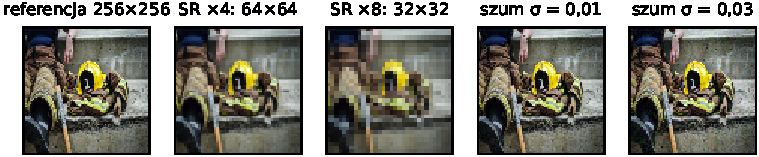
\includegraphics[width=\textwidth]{fig/degradacje.pdf}
  \caption{Przykładowe wejścia dla czterech wariantów (obraz 0721 z naszej walidacji). Wejścia SR są
    pokazane powiększone metodą nearest, żeby było widać prawdziwą liczbę pikseli. Szum $\sigma=0{,}01$
    jest prawie niewidoczny, przy $\sigma=0{,}03$ widać już ziarno na jednolitych powierzchniach.}
  \label{fig:degradacje}
\end{figure}

% ---------------------------------------------------------------- 3
\section{Metody bazowe}\label{sec:bazowe}

\paragraph{Zwiększanie rozdzielczości.} Powiększenie wejścia do $256\times256$ funkcją \code{cv2.resize}
z parametrem \code{interpolation=cv2.INTER\_CUBIC}; wynik przycinamy do $[0,1]$.

\paragraph{Odszumianie.} Funkcja \code{denoise\_bilateral} z modułu \code{skimage.restoration}
z parametrami \code{channel\_axis=-1} i \code{mode="reflect"}. Instrukcja nie podaje parametrów filtru, a domyślne
\code{sigma\_color} w scikit-image jest wyliczane z całego obrazu, co dla tak słabego szumu daje mocne
rozmycie. Żeby porównanie było uczciwe, dobraliśmy parametry na naszym zbiorze walidacyjnym (80 obrazów),
ustawiając \code{sigma\_color}$\,=k\cdot\sigma$ i sprawdzając $k\in\{1,2,3\}$ oraz
\code{sigma\_spatial}$\,\in\{1,3\}$ (tabela~\ref{tab:bilateral}). W obu wariantach wygrało
$k=1$, \code{sigma\_spatial}$\,=3$ i tych wartości używamy w teście.

\begin{table}[H]
  \centering\small
  \caption{Strojenie filtru bilateralnego: średni PSNR [dB] na 80 obrazach walidacyjnych.}
  \label{tab:bilateral}
  \begin{tabular}{@{}l*{3}{S[table-format=2.2]}@{\hspace{1.5em}}*{3}{S[table-format=2.2]}@{}}
    \toprule
    & \multicolumn{3}{c}{$\sigma=0{,}01$} & \multicolumn{3}{c}{$\sigma=0{,}03$} \\
    \cmidrule(lr){2-4}\cmidrule(l){5-7}
    \code{sigma\_color} & {$1\sigma$} & {$2\sigma$} & {$3\sigma$} & {$1\sigma$} & {$2\sigma$} & {$3\sigma$} \\
    \midrule
    \code{sigma\_spatial}$\,=1$ & 36.48 & 32.87 & 30.58 & 30.10 & 26.54 & 24.48 \\
    \code{sigma\_spatial}$\,=3$ & \best{38.93} & 34.80 & 32.01 & \best{31.51} & 27.19 & 24.64 \\
    \bottomrule
  \end{tabular}
\end{table}

Strojenie dużo zmienia -- dla $\sigma=0{,}03$ różnica między najlepszym a najgorszym ustawieniem to
ok.\ 7~dB. Najlepsze $k=1$ leży na brzegu sprawdzanej siatki, więc możliwe, że jeszcze mniejsze
\code{sigma\_color} dałoby trochę lepszy wynik. Tego już nie sprawdzaliśmy.

% ---------------------------------------------------------------- 4
\section{Proponowana architektura: \nazwa}\label{sec:architektura}

Naszą sieć oparliśmy na pomysłach z wykładu W04, głównie z EDSR, VDSR
i DnCNN. Schemat pokazuje rysunek~\ref{fig:architektura}.

\begin{figure}[H]
  \centering
  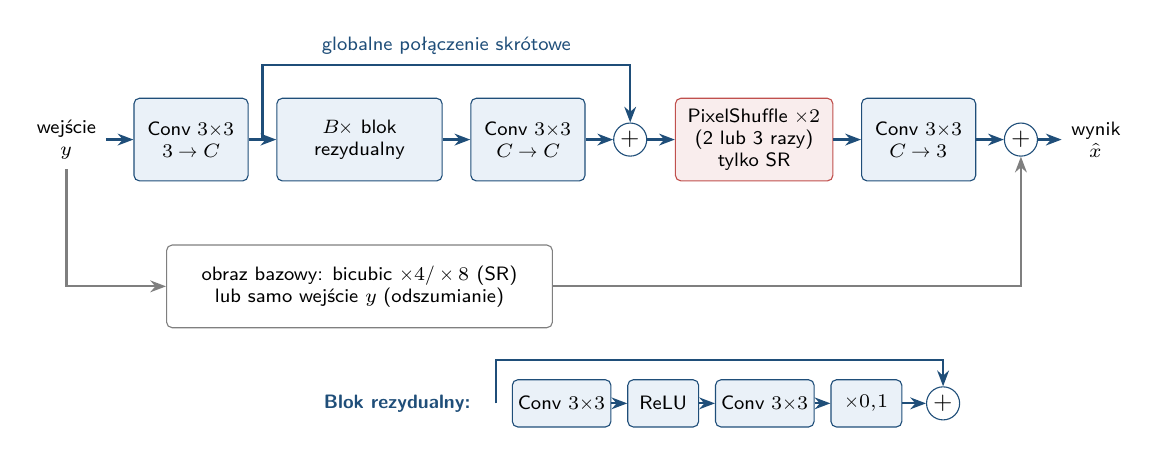
\begin{tikzpicture}[
      font=\sffamily\scriptsize,
      blok/.style={draw=akcent, fill=jasny, rounded corners=2pt, minimum height=1.05cm,
                   minimum width=1.45cm, align=center, inner sep=2pt},
      sr/.style={blok, draw=siec, fill=siec!10},
      wez/.style={circle, draw=akcent, inner sep=0pt, minimum size=4.2mm, font=\sffamily\small},
      strz/.style={-{Stealth[length=2mm]}, thick, color=akcent},
      node distance=3.5mm]
    \node[align=center] (in) {wejście\\$y$};
    \node[blok, right=of in] (head) {Conv $3{\times}3$\\$3\to C$};
    \node[blok, right=of head, minimum width=2.1cm] (res) {$B\times$ blok\\rezydualny};
    \node[blok, right=of res] (conv) {Conv $3{\times}3$\\$C\to C$};
    \node[wez, right=of conv] (plus1) {$+$};
    \node[sr, right=of plus1, minimum width=2.0cm] (up) {PixelShuffle $\times2$\\(2 lub 3 razy)\\tylko SR};
    \node[blok, right=of up] (tail) {Conv $3{\times}3$\\$C\to 3$};
    \node[wez, right=of tail] (plus2) {$+$};
    \node[right=3mm of plus2, align=center] (out) {wynik\\$\hat{x}$};
    \draw[strz] (in) -- (head);
    \draw[strz] (head) -- (res);
    \draw[strz] (res) -- (conv);
    \draw[strz] (conv) -- (plus1);
    \draw[strz] (plus1) -- (up);
    \draw[strz] (up) -- (tail);
    \draw[strz] (tail) -- (plus2);
    \draw[strz] (plus2) -- (out);
    \draw[strz] ($(head.east)!0.5!(res.west)$) -- ++(0,0.95) -| node[pos=0.25, above]{globalne połączenie skrótowe} (plus1);
    \node[blok, draw=baza, fill=white, below=8mm of res, minimum width=4.9cm] (base)
      {obraz bazowy: bicubic $\times4/\times8$ (SR)\\lub samo wejście $y$ (odszumianie)};
    \draw[strz, color=baza] (in) |- (base);
    \draw[strz, color=baza] (base) -| (plus2);
    % blok rezydualny
    \begin{scope}[shift={(4.2,-3.35)}]
      \node[font=\sffamily\scriptsize\bfseries, color=akcent] (lab) at (0,0) {Blok rezydualny:};
      \node[blok, right=4mm of lab, minimum height=0.6cm, minimum width=1.2cm] (c1) {Conv $3{\times}3$};
      \node[blok, right=2mm of c1, minimum height=0.6cm, minimum width=0.9cm] (r) {ReLU};
      \node[blok, right=2mm of r, minimum height=0.6cm, minimum width=1.2cm] (c2) {Conv $3{\times}3$};
      \node[blok, right=2mm of c2, minimum height=0.6cm, minimum width=0.9cm] (sc) {$\times0{,}1$};
      \node[wez, right=3mm of sc] (p) {$+$};
      \draw[strz] (c1) -- (r); \draw[strz] (r) -- (c2); \draw[strz] (c2) -- (sc); \draw[strz] (sc) -- (p);
      \draw[strz] ($(lab.east)!0.5!(c1.west)$) -- ++(0,0.55) -| (p);
    \end{scope}
  \end{tikzpicture}
  \caption{Architektura \nazwa. Na niebiesko część wspólna dla obu zadań, na czerwono moduł powiększania
    używany tylko w SR. Sieć przewiduje poprawkę, którą dodajemy do obrazu bazowego. W SR większość obliczeń
    odbywa się w niskiej rozdzielczości, a powiększenie jest dopiero na końcu.}
  \label{fig:architektura}
\end{figure}

Najważniejsze decyzje projektowe:
\begin{itemize}
  \item \textbf{Uczenie poprawki (residual learning).} Sieć nie generuje całego obrazu, tylko różnicę
        względem obrazu bazowego: $\hat{x} = \text{baza}(y) + r_\theta(y)$. W SR bazą jest wynik bicubic,
        a w odszumianiu sam zaszumiony obraz. To ten sam pomysł co w VDSR i DnCNN.
  \item \textbf{Zerowa inicjalizacja ostatniej warstwy.} Na starcie $r_\theta(y)=0$, czyli nieuczona sieć
        daje dokładnie wynik bicubic (SR) lub zwraca wejście bez zmian (odszumianie). Trening zaczyna się więc
        od poziomu metody bazowej i ma ją tylko poprawiać.
  \item \textbf{Bloki rezydualne bez BatchNorm} -- jak w EDSR. Brak normalizacji nie zaburza zakresu
        jasności obrazu, a mnożenie wyjścia bloku przez $0{,}1$ stabilizuje uczenie.
  \item \textbf{PixelShuffle na końcu (tylko SR).} Cechy liczymy dla obrazu $64\times64$ lub $32\times32$,
        a powiększamy je dopiero na końcu: dwa kroki $\times2$ dla $\times4$ i trzy dla $\times8$.
        Jest to dużo tańsze niż przetwarzanie obrazu $256\times256$ przez całą sieć.
  \item \textbf{Mała sieć:} $C=24$ kanały i $B=4$ bloki. Chcieliśmy, żeby cały eksperyment (4 modele)
        dało się wytrenować w kilkanaście minut na laptopie, i okazało się, że to wystarcza, żeby pokonać
        metody bazowe.
\end{itemize}

\begin{table}[H]
  \centering\small
  \caption{Liczba parametrów modeli (dla porównania EDSR ma ok.\ 43~mln parametrów).}
  \label{tab:parametry}
  \begin{tabular}{@{}lccr@{}}
    \toprule
    Wariant & Wejście & Moduł powiększania & Parametry \\
    \midrule
    \code{sr4}            & $64\times64$   & $2\times$ PixelShuffle $\times2$ & \num{89859} \\
    \code{sr8}            & $32\times32$   & $3\times$ PixelShuffle $\times2$ & \num{110691} \\
    \code{dn001}, \code{dn003} & $256\times256$ & brak & \num{48195} \\
    \bottomrule
  \end{tabular}
\end{table}

% ---------------------------------------------------------------- 5
\section{Trening}\label{sec:trening}

Wszystkie cztery modele trenowaliśmy z tymi samymi ustawieniami (tabela~\ref{tab:trening}).
Funkcją straty było MSE, bo PSNR zależy bezpośrednio od MSE. EDSR używa straty L1, ale tego wariantu
nie porównywaliśmy (patrz sekcja~\ref{sec:ograniczenia}). Po każdej epoce liczymy średni PSNR na
zbiorze walidacyjnym i zapisujemy model z najlepszym wynikiem (\code{best.pt}).

\begin{table}[H]
  \centering\small
  \caption{Ustawienia treningu (takie same dla wszystkich wariantów).}
  \label{tab:trening}
  \begin{tabularx}{\textwidth}{@{}lX@{}}
    \toprule
    Optymalizator & Adam, $\text{lr}=10^{-3}$, harmonogram kosinusowy do $10^{-5}$, przycinanie gradientu do normy 1 \\
    Epoki, batch & 30 epok, batch 8; każdy obraz treningowy 2 razy na epokę (1440 próbek) \\
    Augmentacja & losowy obrót o wielokrotność $90^\circ$ i odbicie poziome; w odszumianiu nowy szum w każdej epoce \\
    Strata & MSE na obrazie RGB w zakresie $[0,1]$, bez obcinania wyniku w trakcie treningu \\
    Precyzja & SR: FP32; odszumianie: BF16 (autocast), wagi i optymalizator w FP32; walidacja zawsze FP32 \\
    Wybór modelu & najlepszy średni PSNR na walidacji (80 obrazów) \\
    Sprzęt & NVIDIA RTX 5080 Laptop GPU, PyTorch 2.10.0, CUDA 12.8, ziarno 42 \\
    \bottomrule
  \end{tabularx}
\end{table}

\begin{table}[H]
  \centering\small
  \caption{Czas treningu i wybrane epoki.}
  \label{tab:czasy}
  \begin{tabular}{@{}lS[table-format=3.0]S[table-format=2.1]cS[table-format=2.2]S[table-format=2.2]@{}}
    \toprule
    Wariant & {Czas [s]} & {s/epokę} & {Wybrana epoka} & {PSNR wal., ep.\,1 [dB]} & {PSNR wal., najlepszy [dB]} \\
    \midrule
    \code{sr4}   & 122 & 4.1  & 29 & 24.10 & 24.47 \\
    \code{sr8}   & 168 & 5.6  & 28 & 21.24 & 21.46 \\
    \code{dn001} & 302 & 10.1 & 30 & 40.37 & 42.65 \\
    \code{dn003} & 303 & 10.1 & 29 & 33.41 & 36.18 \\
    \bottomrule
  \end{tabular}
\end{table}

\begin{figure}[H]
  \centering
  \begin{tikzpicture}
    \begin{groupplot}[group style={group size=4 by 1, horizontal sep=1.15cm},
        width=4.4cm, height=4.0cm, xmin=1, xmax=30, xtick={1,10,20,30},
        xlabel={epoka}, grid=major, grid style={gray!25},
        tick label style={font=\scriptsize}, label style={font=\scriptsize},
        title style={font=\small\sffamily, yshift=-1mm},
        /pgf/number format/use comma, every axis plot/.style={thick, color=akcent, mark=none}]
      \nextgroupplot[title={\code{sr4}}, ylabel={PSNR walidacji [dB]},
        yticklabel style={/pgf/number format/fixed, /pgf/number format/precision=1}]
        \addplot table[x=epoch, y=val_PSNR, col sep=comma] {../../runs/main/sr4/history.csv};
      \nextgroupplot[title={\code{sr8}},
        yticklabel style={/pgf/number format/fixed, /pgf/number format/precision=2}]
        \addplot table[x=epoch, y=val_PSNR, col sep=comma] {../../runs/main/sr8/history.csv};
      \nextgroupplot[title={\code{dn001}}]
        \addplot table[x=epoch, y=val_PSNR, col sep=comma] {../../runs/main/dn001/history.csv};
      \nextgroupplot[title={\code{dn003}}]
        \addplot table[x=epoch, y=val_PSNR, col sep=comma] {../../runs/main/dn003/history.csv};
    \end{groupplot}
  \end{tikzpicture}
  \caption{PSNR na zbiorze walidacyjnym po każdej epoce (dane z \code{runs/main/*/history.csv}).}
  \label{fig:krzywe}
\end{figure}

Na krzywych (rys.~\ref{fig:krzywe}) widać, że modele SR uczą się szybko i od ok.\ 20.~epoki wynik
prawie się nie zmienia -- zysk w całym treningu to tylko ok.\ $0{,}2$--$0{,}4$~dB, ale zaczynamy już
od poziomu bicubic. Modele odszumiające poprawiają się dużo bardziej (o $2{,}3$ i $2{,}8$~dB) i jeszcze
pod koniec minimalnie rosną, więc dłuższy trening mógłby im trochę pomóc.

\subsection{Eksperyment: FP32 czy BF16?}

Trening odszumiania był najwolniejszy, bo sieć pracuje na obrazach $256\times256$. Sprawdziliśmy więc,
czy możemy przyspieszyć go obliczeniami w BF16 bez utraty jakości. Uruchomiliśmy model \code{dn001}
w FP32 i w BF16 z tym samym ziarnem i tym samym (CPU) generatorem szumu, a potem przenieśliśmy
generowanie szumu na GPU. Wyniki pierwszych 4 epok są w tabeli~\ref{tab:bf16} (logi w \code{runs/preliminary}).

\begin{table}[H]
  \centering\small
  \caption{PSNR walidacji [dB] i czas epoki [s] dla \code{dn001} przy różnych ustawieniach precyzji.}
  \label{tab:bf16}
  \begin{tabular}{@{}l*{4}{S[table-format=2.3]}S[table-format=2.1]@{}}
    \toprule
    Ustawienie & {Ep.~1} & {Ep.~2} & {Ep.~3} & {Ep.~4} & {Śr. czas epoki} \\
    \midrule
    FP32, szum na CPU         & 40.346 & 40.599 & 40.854 & 41.064 & 23.2 \\
    BF16, szum na CPU         & 40.347 & 40.601 & 40.855 & 41.062 & 16.4 \\
    BF16, szum na GPU (końcowy) & 40.372 & 40.661 & 40.988 & 41.160 & 9.7 \\
    \bottomrule
  \end{tabular}
\end{table}

Przy tym samym szumie FP32 i BF16 różnią się o mniej niż $0{,}003$~dB, więc BF16 nie psuje jakości.
Przeniesienie losowania szumu na GPU skróciło epokę jeszcze ok.\ $1{,}7$ raza (wcześniej procesor
nie nadążał z przygotowaniem danych). Ostatni wiersz różni się trochę od pozostałych, bo generator
na GPU losuje inne realizacje szumu. Te ustawienia przyjęliśmy dla końcowych modeli odszumiających.

% ---------------------------------------------------------------- 6
\section{Metryki}\label{sec:metryki}

Zgodnie z instrukcją używamy wszystkich metryk z wykładu W03. $Y_1$ to obraz referencyjny, $Y_2$ wynik
metody, a $N = 256\cdot256\cdot3 = \num{196608}$ to liczba wartości w obrazie RGB.

\begin{itemize}
  \item \textbf{SNE} (Squared Norm Error, niższe lepsze) -- suma kwadratów różnic pikseli:
        \[ \text{SNE} = \sum (Y_1 - Y_2)^2 . \]
        Liczymy ją dla obrazów w zakresie $[0,1]$, po wszystkich pikselach i kanałach. W skali $0$--$255$
        wartości byłyby $255^2$ razy większe.
  \item \textbf{PSNR} (wyższe lepsze):
        \[ \text{PSNR} = 10\log_{10}\frac{\text{MAX}^2}{\text{MSE}}, \qquad \text{MSE} = \frac{1}{N}\sum(Y_1-Y_2)^2, \qquad \text{MAX}=1 . \]
  \item \textbf{SSIM} (wyższe lepsze) -- funkcja \code{structural\_similarity}
        z modułu \code{skimage.metrics}, okno gaussowskie $\sigma=1{,}5$, \code{data\_range=1},
        liczone dla każdego kanału RGB i uśrednione.
  \item \textbf{LPIPS} (niższe lepsze) -- biblioteka \code{lpips} 0.1.4, wersja 0.1,
        sieć SqueezeNet z wytrenowanymi wagami, obrazy przeskalowane do $[-1,1]$.
\end{itemize}

Metryki liczymy dla każdego obrazu osobno, na pełnym obrazie $256\times256$ (bez obcinania brzegów),
na wartościach \code{float} jeszcze przed zapisem do PNG. W tabelach podajemy średnią z wszystkich
100 obrazów testowych. Warto zauważyć, że dla jednego obrazu SNE i PSNR niosą tę samą informację
($\text{PSNR} = 10\log_{10}(N/\text{SNE})$), ale po uśrednieniu po obrazach już nie: na średnie SNE
mocno wpływają najtrudniejsze obrazy z dużym błędem. Wartości LPIPS dla SqueezeNet nie należy porównywać
wprost z artykułami, w których używano AlexNet.

% ---------------------------------------------------------------- 7
\section{Wyniki}\label{sec:wyniki}

Wszystkie wyniki pochodzą z pełnej ewaluacji na 100 obrazach testowych. Średnie są zapisane
w pliku \code{runs/evaluation/summary.csv}, a wyniki każdego obrazu w \code{per\_image.csv}
w tym samym katalogu. Najlepszy wynik w każdym wariancie jest pogrubiony.

\subsection{Zwiększanie rozdzielczości}

\begin{table}[H]
  \centering\small
  \caption{Zwiększanie rozdzielczości do $256\times256$, zbiór testowy DIV2K (100 obrazów).
    Wejście zmniejszone przez \code{cv2.resize} z \code{INTER\_AREA}. $\uparrow$ -- wyższe lepsze, $\downarrow$ -- niższe lepsze.}
  \label{tab:wyniki-sr}
  \begin{tabular}{@{}lS[table-format=2.2]S[table-format=1.4]S[table-format=1.4]S[table-format=4.1]@{}}
    \toprule
    Metoda & {PSNR [dB] $\uparrow$} & {SSIM $\uparrow$} & {LPIPS $\downarrow$} & {SNE $\downarrow$} \\
    \midrule
    bicubic OpenCV, SR $\times4$ ($64\times64\to256\times256$)     & 22.91 & 0.6445 & 0.3978 & 1216.2 \\
    \nazwa, SR $\times4$ ($64\times64\to256\times256$)             & \best{23.63} & \best{0.6898} & \best{0.2886} & \best{1055.0} \\
    \midrule
    bicubic OpenCV, SR $\times8$ ($32\times32\to256\times256$)     & 20.30 & 0.4673 & 0.7355 & 2148.5 \\
    \nazwa, SR $\times8$ ($32\times32\to256\times256$)             & \best{20.75} & \best{0.5001} & \best{0.5990} & \best{1962.0} \\
    \bottomrule
  \end{tabular}
\end{table}

\subsection{Odszumianie}

\begin{table}[H]
  \centering\small
  \caption{Odszumianie obrazów $256\times256$ z szumem gaussowskim, zbiór testowy DIV2K (100 obrazów).
    Dla porównania dodaliśmy wiersz z samym zaszumionym wejściem (bez żadnej filtracji).}
  \label{tab:wyniki-dn}
  \begin{tabular}{@{}lS[table-format=2.2]S[table-format=1.4]S[table-format=1.4]S[table-format=3.1]@{}}
    \toprule
    Metoda & {PSNR [dB] $\uparrow$} & {SSIM $\uparrow$} & {LPIPS $\downarrow$} & {SNE $\downarrow$} \\
    \midrule
    wejście zaszumione, szum gaussowski $\sigma=0{,}01$            & 40.07 & 0.9709 & 0.0179 & 19.4 \\
    denoise bilateral, szum gaussowski $\sigma=0{,}01$             & 38.79 & 0.9816 & 0.0143 & 27.5 \\
    \nazwa, szum gaussowski $\sigma=0{,}01$                         & \best{42.56} & \best{0.9881} & \best{0.0115} & \best{11.1} \\
    \midrule
    wejście zaszumione, szum gaussowski $\sigma=0{,}03$            & 30.60 & 0.8285 & 0.1009 & 171.6 \\
    denoise bilateral, szum gaussowski $\sigma=0{,}03$             & 31.35 & 0.9192 & 0.0608 & 152.8 \\
    \nazwa, szum gaussowski $\sigma=0{,}03$                         & \best{36.01} & \best{0.9664} & \best{0.0221} & \best{52.2} \\
    \bottomrule
  \end{tabular}
\end{table}

\subsection{Wyniki dla pojedynczych obrazów}

Same średnie mogą ukrywać to, że na części obrazów sieć wypada gorzej. Dlatego policzyliśmy, na ilu
obrazach testowych sieć jest lepsza od metody bazowej w każdej metryce, oraz jak rozkłada się różnica
PSNR (tabela~\ref{tab:obrazy}).

\begin{table}[H]
  \centering\small
  \caption{Porównanie \nazwa{} z metodą bazową na pojedynczych obrazach testowych (na 100).
    $\Delta$PSNR = PSNR sieci $-$ PSNR metody bazowej.}
  \label{tab:obrazy}
  \begin{tabular}{@{}l*{4}{c}S[table-format=1.2]S[table-format=-1.2]S[table-format=1.2]@{}}
    \toprule
    & \multicolumn{4}{c}{Sieć lepsza na \ldots{} obrazach} & \multicolumn{3}{c}{$\Delta$PSNR [dB]} \\
    \cmidrule(lr){2-5}\cmidrule(l){6-8}
    Wariant & PSNR & SSIM & LPIPS & SNE & {mediana} & {min.} & {maks.} \\
    \midrule
    SR $\times4$             & 100 & 100 & 100 & 100 & 0.57 & 0.10 & 2.94 \\
    SR $\times8$             & 100 & 100 & 100 & 100 & 0.36 & 0.05 & 2.39 \\
    szum $\sigma=0{,}01$     & 99  & 87  & 78  & 99  & 3.90 & -0.73 & 5.98 \\
    szum $\sigma=0{,}03$     & 100 & 100 & 95  & 100 & 4.60 & 1.88 & 7.55 \\
    \bottomrule
  \end{tabular}
\end{table}

W SR sieć jest lepsza na każdym obrazie testowym, chociaż na niektórych zysk jest bardzo mały
($0{,}05$~dB). Przy słabym szumie ($\sigma=0{,}01$) jest jeden obraz (0868), na którym filtr bilateralny
dał wyższy PSNR, a w SSIM i LPIPS sieć przegrywa odpowiednio na 13 i 22 obrazach. Przy tak słabym szumie
filtr bilateralny prawie nic nie zmienia na jednolitych fragmentach, a sieć czasem lekko wygładza drobne
tekstury -- PSNR to wybacza, ale metryki strukturalne i percepcyjne już nie.

\subsection{Wyniki wizualne}\label{sec:wizualne}

Rysunki~\ref{fig:sr}--\ref{fig:mapy} pokazują ten sam fragment obrazu 0721 (z naszej walidacji) dla wszystkich
metod. Wartości PSNR w tytułach dotyczą całego obrazu zapisanego jako 8-bitowy PNG, więc mogą się trochę
różnić od wartości liczonych na danych \code{float}. Porównania z mapami błędu dla obrazów testowych są
w dodatku~\ref{sec:dodatek} i w raporcie \code{runs/evaluation/raport.html}.

\begin{figure}[H]
  \centering
  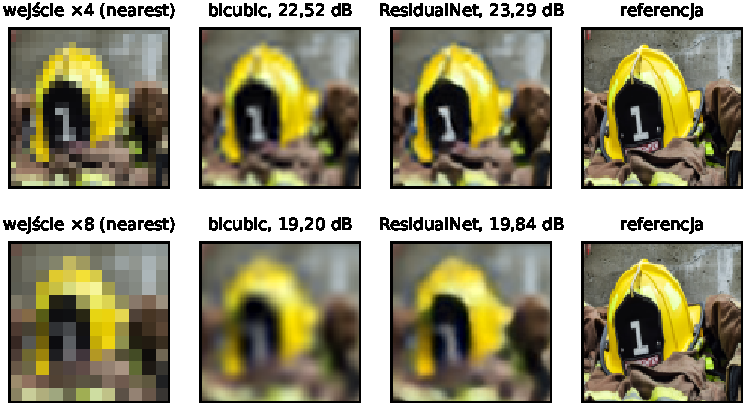
\includegraphics[width=\textwidth]{fig/sr_porownanie.pdf}
  \caption{Zwiększanie rozdzielczości, wycinek $96\times96$. Sieć daje wyraźniejsze krawędzie kasku i cyfry
    \enquote{1} niż bicubic. Przy $\times8$ obu metodom brakuje szczegółów -- z obrazu $32\times32$ nie da się
    ich odtworzyć, a sieć uczona na MSE woli bezpieczne, lekko rozmyte przewidywania.}
  \label{fig:sr}
\end{figure}

\begin{figure}[H]
  \centering
  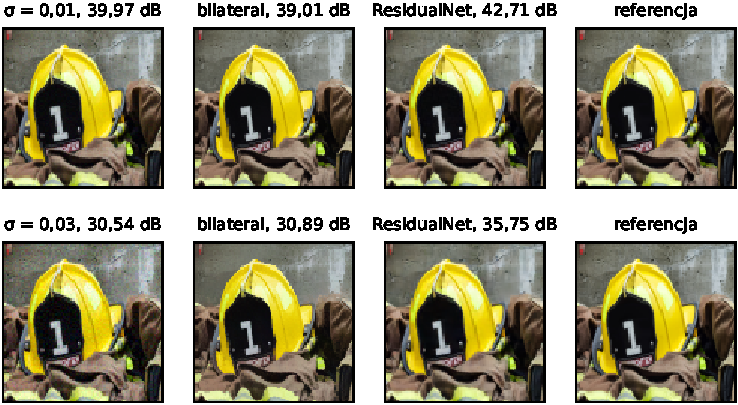
\includegraphics[width=\textwidth]{fig/dn_porownanie.pdf}
  \caption{Odszumianie, wycinek $96\times96$. Przy $\sigma=0{,}01$ szum jest prawie niewidoczny, a filtr
    bilateralny obniża PSNR względem samego wejścia, bo rusza też szczegóły obrazu. Przy $\sigma=0{,}03$ sieć
    usuwa ziarno na kasku i tle, zachowując ostre krawędzie.}
  \label{fig:dn}
\end{figure}

\begin{figure}[H]
  \centering
  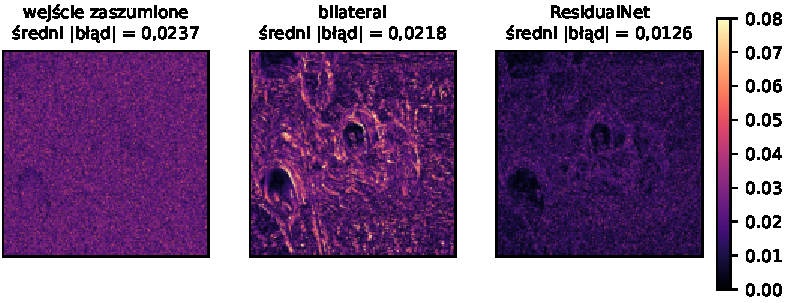
\includegraphics[width=0.92\textwidth]{fig/dn_mapy_bledu.pdf}
  \caption{Mapy średniego błędu bezwzględnego RGB dla $\sigma=0{,}03$ (cały obraz). Błąd zaszumionego wejścia
    jest równomierny. Filtr bilateralny zmniejsza go na gładkich powierzchniach, ale tworzy duże błędy na
    teksturach (materiał kurtki, beton). Błąd sieci jest najmniejszy i skupia się głównie na krawędziach.}
  \label{fig:mapy}
\end{figure}

% ---------------------------------------------------------------- 8
\section{Wnioski}\label{sec:wnioski}

\begin{enumerate}
  \item \textbf{Mała sieć wystarczyła, żeby pokonać metody bazowe.} \nazwa{} ma 48--111 tys.\ parametrów
        i trenuje się od 2 do 5 minut na model, a mimo to we wszystkich czterech wariantach jest lepsza od bicubic
        i od dostrojonego filtru bilateralnego w każdej z metryk SNE, PSNR, SSIM i LPIPS.
  \item \textbf{Odszumianie zyskało dużo więcej niż SR} ($+3{,}8$ / $+4{,}7$~dB wobec $+0{,}7$ / $+0{,}5$~dB).
        Szum jest losowy i niezależny od treści obrazu, więc sieć łatwo go odróżnia od krawędzi i tekstur.
        W SR informacja usunięta przy zmniejszaniu jest tracona na stałe -- to problem odwrotny z wykładu W04,
        w którym wiele obrazów HR daje ten sam obraz LR. Przy $\times8$ tracimy 98\% pikseli, więc zysk jest najmniejszy.
  \item \textbf{W SR LPIPS poprawił się bardziej, niż sugeruje PSNR.} Przy $\times4$ LPIPS spadł z $0{,}398$ do
        $0{,}289$ (o 27\%), a PSNR wzrósł tylko o $0{,}7$~dB. Obrazy wyglądają więc wyraźnie lepiej, mimo
        niewielkiej poprawy w metrykach pikselowych.
  \item \textbf{Metryki nie zawsze się zgadzają.} Filtr bilateralny przy $\sigma=0{,}01$ obniża PSNR względem
        samego wejścia ($40{,}07\to38{,}79$~dB), ale poprawia SSIM i LPIPS. Dla tego samego wariantu sieć wygrywa
        w PSNR na 99 obrazach, a w LPIPS tylko na 78. Pokazuje to kompromis między dokładnością pikselową a jakością
        percepcyjną (perception--distortion trade-off), dlatego warto patrzeć na kilka metryk naraz.
  \item \textbf{Metoda klasyczna jest bardzo wrażliwa na parametry.} Wybór \code{sigma\_color} zmieniał wynik
        filtru bilateralnego nawet o 7~dB. Bez strojenia przewaga sieci byłaby dużo większa, ale wtedy porównanie
        nie byłoby uczciwe.
  \item \textbf{BF16 przyspiesza trening bez utraty jakości.} Razem z generowaniem szumu na GPU trening odszumiania
        był ok.\ 2,4 raza szybszy niż w FP32 z szumem na CPU.
\end{enumerate}

% ---------------------------------------------------------------- 9
\section{Ograniczenia i co można by zrobić dalej}\label{sec:ograniczenia}

\begin{itemize}
  \item \textbf{Zbiór testowy.} Używamy oficjalnej walidacji DIV2K (0801--0900), bo referencje oficjalnego
        testu nie są publiczne. Kod pozwala podmienić zbiór testowy (\code{prepare --test-dir}), gdyby udało się
        go zdobyć.
  \item \textbf{Jeden trening na wariant.} Każdy model trenowaliśmy raz, z jednym ziarnem, więc nie wiemy, jak
        bardzo wyniki zależą od losowości. Przy SR $\times8$, gdzie zysk wynosi $0{,}45$~dB, warto by to sprawdzić.
  \item \textbf{Mała sieć i krótki trening.} Modele odszumiające jeszcze się poprawiały w 30.~epoce. Następnym
        krokiem byłaby większa sieć (np. 32 kanały, 6 bloków) i 60 epok -- kod już to obsługuje.
  \item \textbf{Inna funkcja straty.} EDSR uczy się z L1, a SRGAN/ESRGAN ze stratą percepcyjną. Strata L1
        (\code{train --loss l1}) mogłaby poprawić LPIPS kosztem PSNR.
  \item \textbf{Proporcje obrazu.} Cały obraz skalujemy do kwadratu, więc obiekty są lekko zniekształcone.
        Alternatywą byłoby wycinanie kwadratowego fragmentu, ale wtedy część obrazu nie trafiłaby do testu.
\end{itemize}

% ---------------------------------------------------------------- 10
\section{Jak uruchomić}

Instalacja: \code{python -m pip install -r requirements.txt} (Python $\geq$ 3.10). Najważniejsze komendy:
\begin{center}\small
\begin{tabularx}{\textwidth}{@{}l>{\raggedright\arraybackslash}X@{}}
  \toprule
  \code{python -m src download}, \code{prepare}, \code{verify} & pobranie DIV2K, przygotowanie $256\times256$, kontrola danych \\
  \code{python -m src train --condition sr4} & trening jednego wariantu (\code{sr4}, \code{sr8}, \code{dn001}, \code{dn003}) \\
  \code{python -m src tune-baseline} & strojenie filtru bilateralnego na walidacji \\
  \code{python -m src evaluate --sne-definition sse ...} & pełna ewaluacja i raport HTML \\
  \code{python -m src predict --checkpoint ... --input ...} & przetworzenie własnego obrazu \\
  \bottomrule
\end{tabularx}
\end{center}
Pełny opis i polecenia odtwarzające cały eksperyment znajdują się w \code{README.md}.
Rysunki do tego sprawozdania generuje \code{docs/sprawozdanie/make\_figures.py}.

% ---------------------------------------------------------------- dodatek
\appendix
\section{Przykłady z raportu dla obrazów testowych}\label{sec:dodatek}

Poniższe rysunki pochodzą z raportu wygenerowanego podczas ewaluacji. Górny wiersz: referencja, wejście,
metoda bazowa i \nazwa. Dolny wiersz: powiększony wycinek referencji i mapy średniego błędu RGB (skala 0--0,1).
W SR kolumna \enquote{wejście} pokazuje obraz już powiększony metodą bicubic, więc jest taka sama jak kolumna
metody bazowej. Wszystkie 20 porównań (po 5 na wariant) jest w \code{runs/evaluation/images}.

\begin{figure}[H]
  \centering
  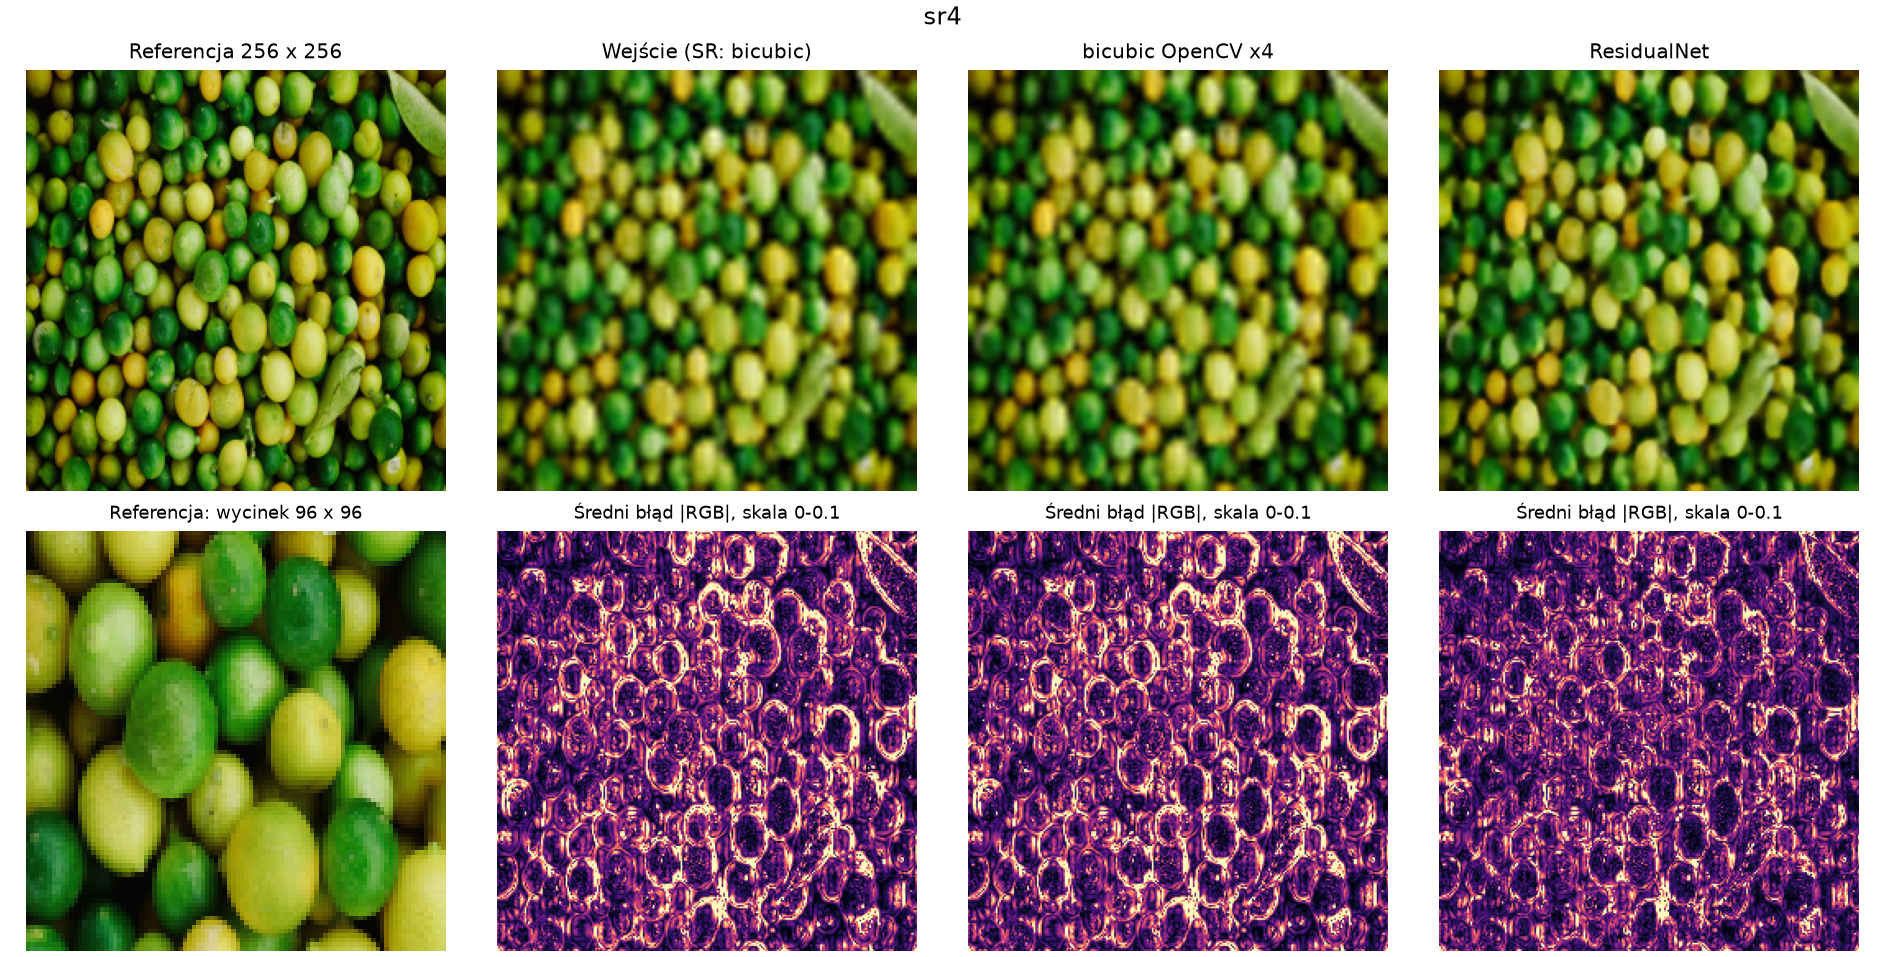
\includegraphics[width=\textwidth]{../../runs/evaluation/images/sr4_0802.png}
  \caption{SR $\times4$, obraz testowy 0802 (PSNR: bicubic 24,39~dB, \nazwa{} 25,69~dB).}
\end{figure}

\begin{figure}[H]
  \centering
  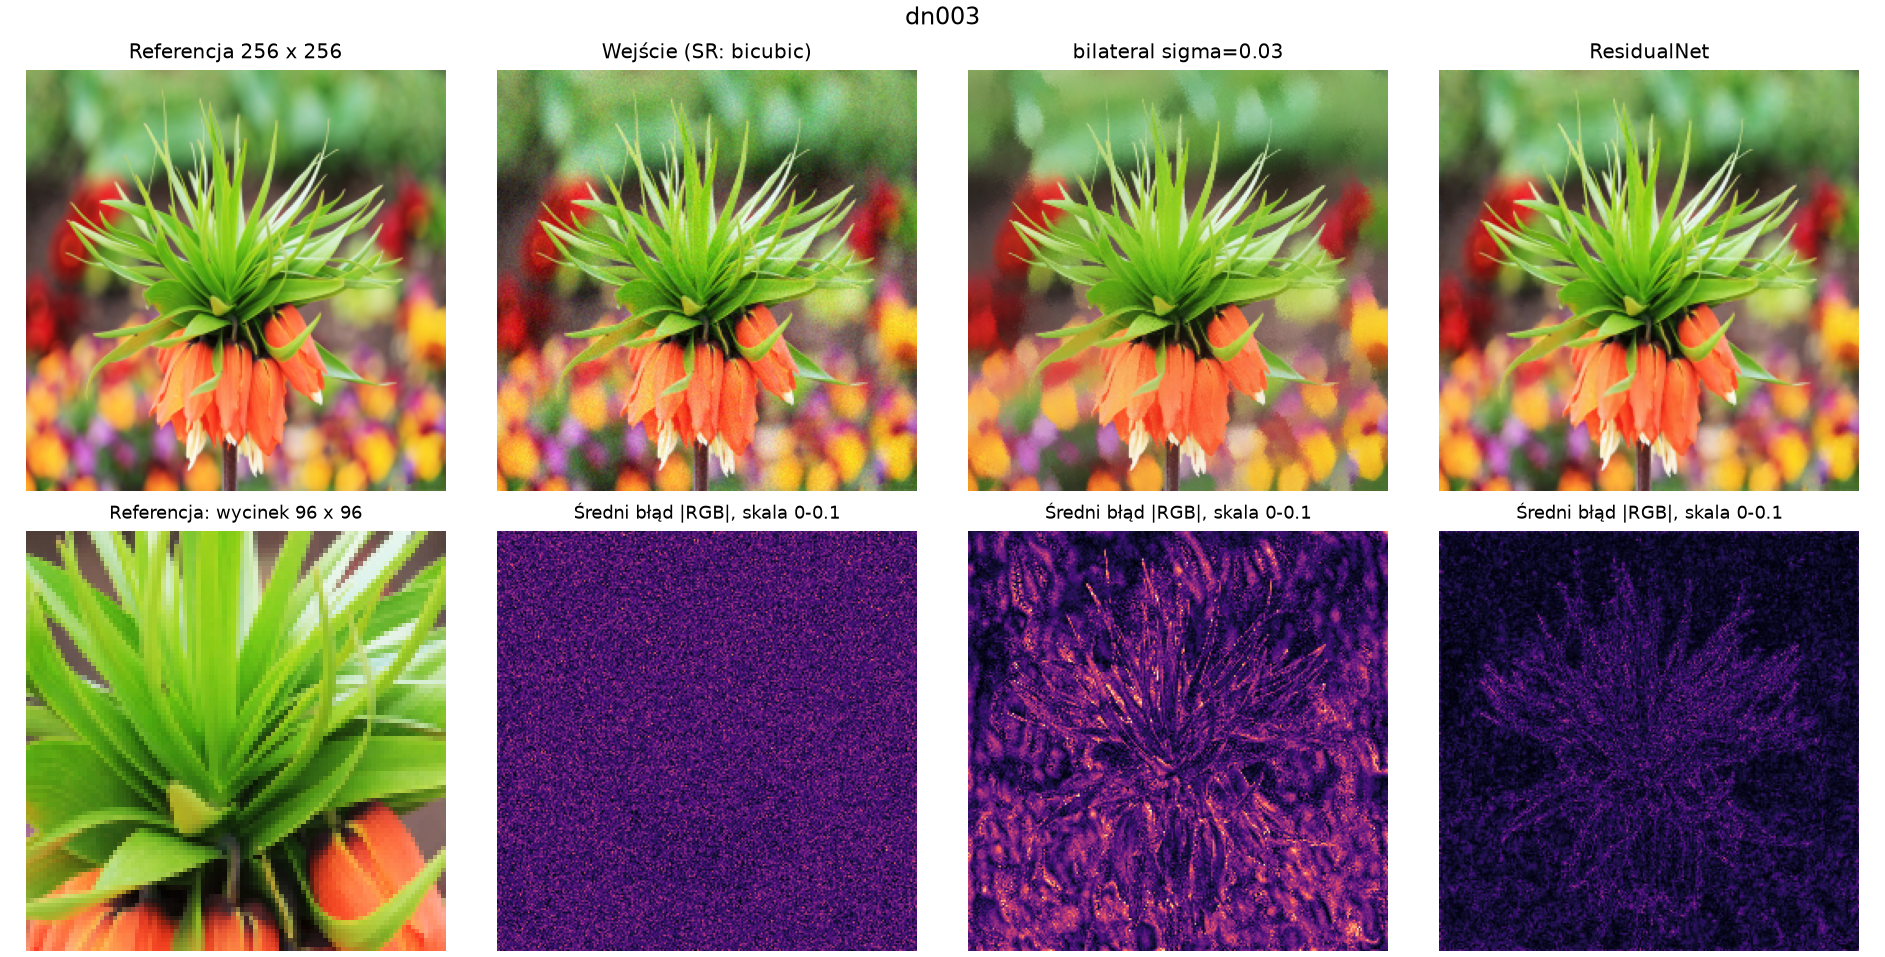
\includegraphics[width=\textwidth]{../../runs/evaluation/images/dn003_0803.png}
  \caption{Odszumianie $\sigma=0{,}03$, obraz testowy 0803 (PSNR: bilateral 29,24~dB, \nazwa{} 36,33~dB).}
\end{figure}

\end{document}
